% !TeX spellcheck = en

\begin{figure}
	\begin{center}
		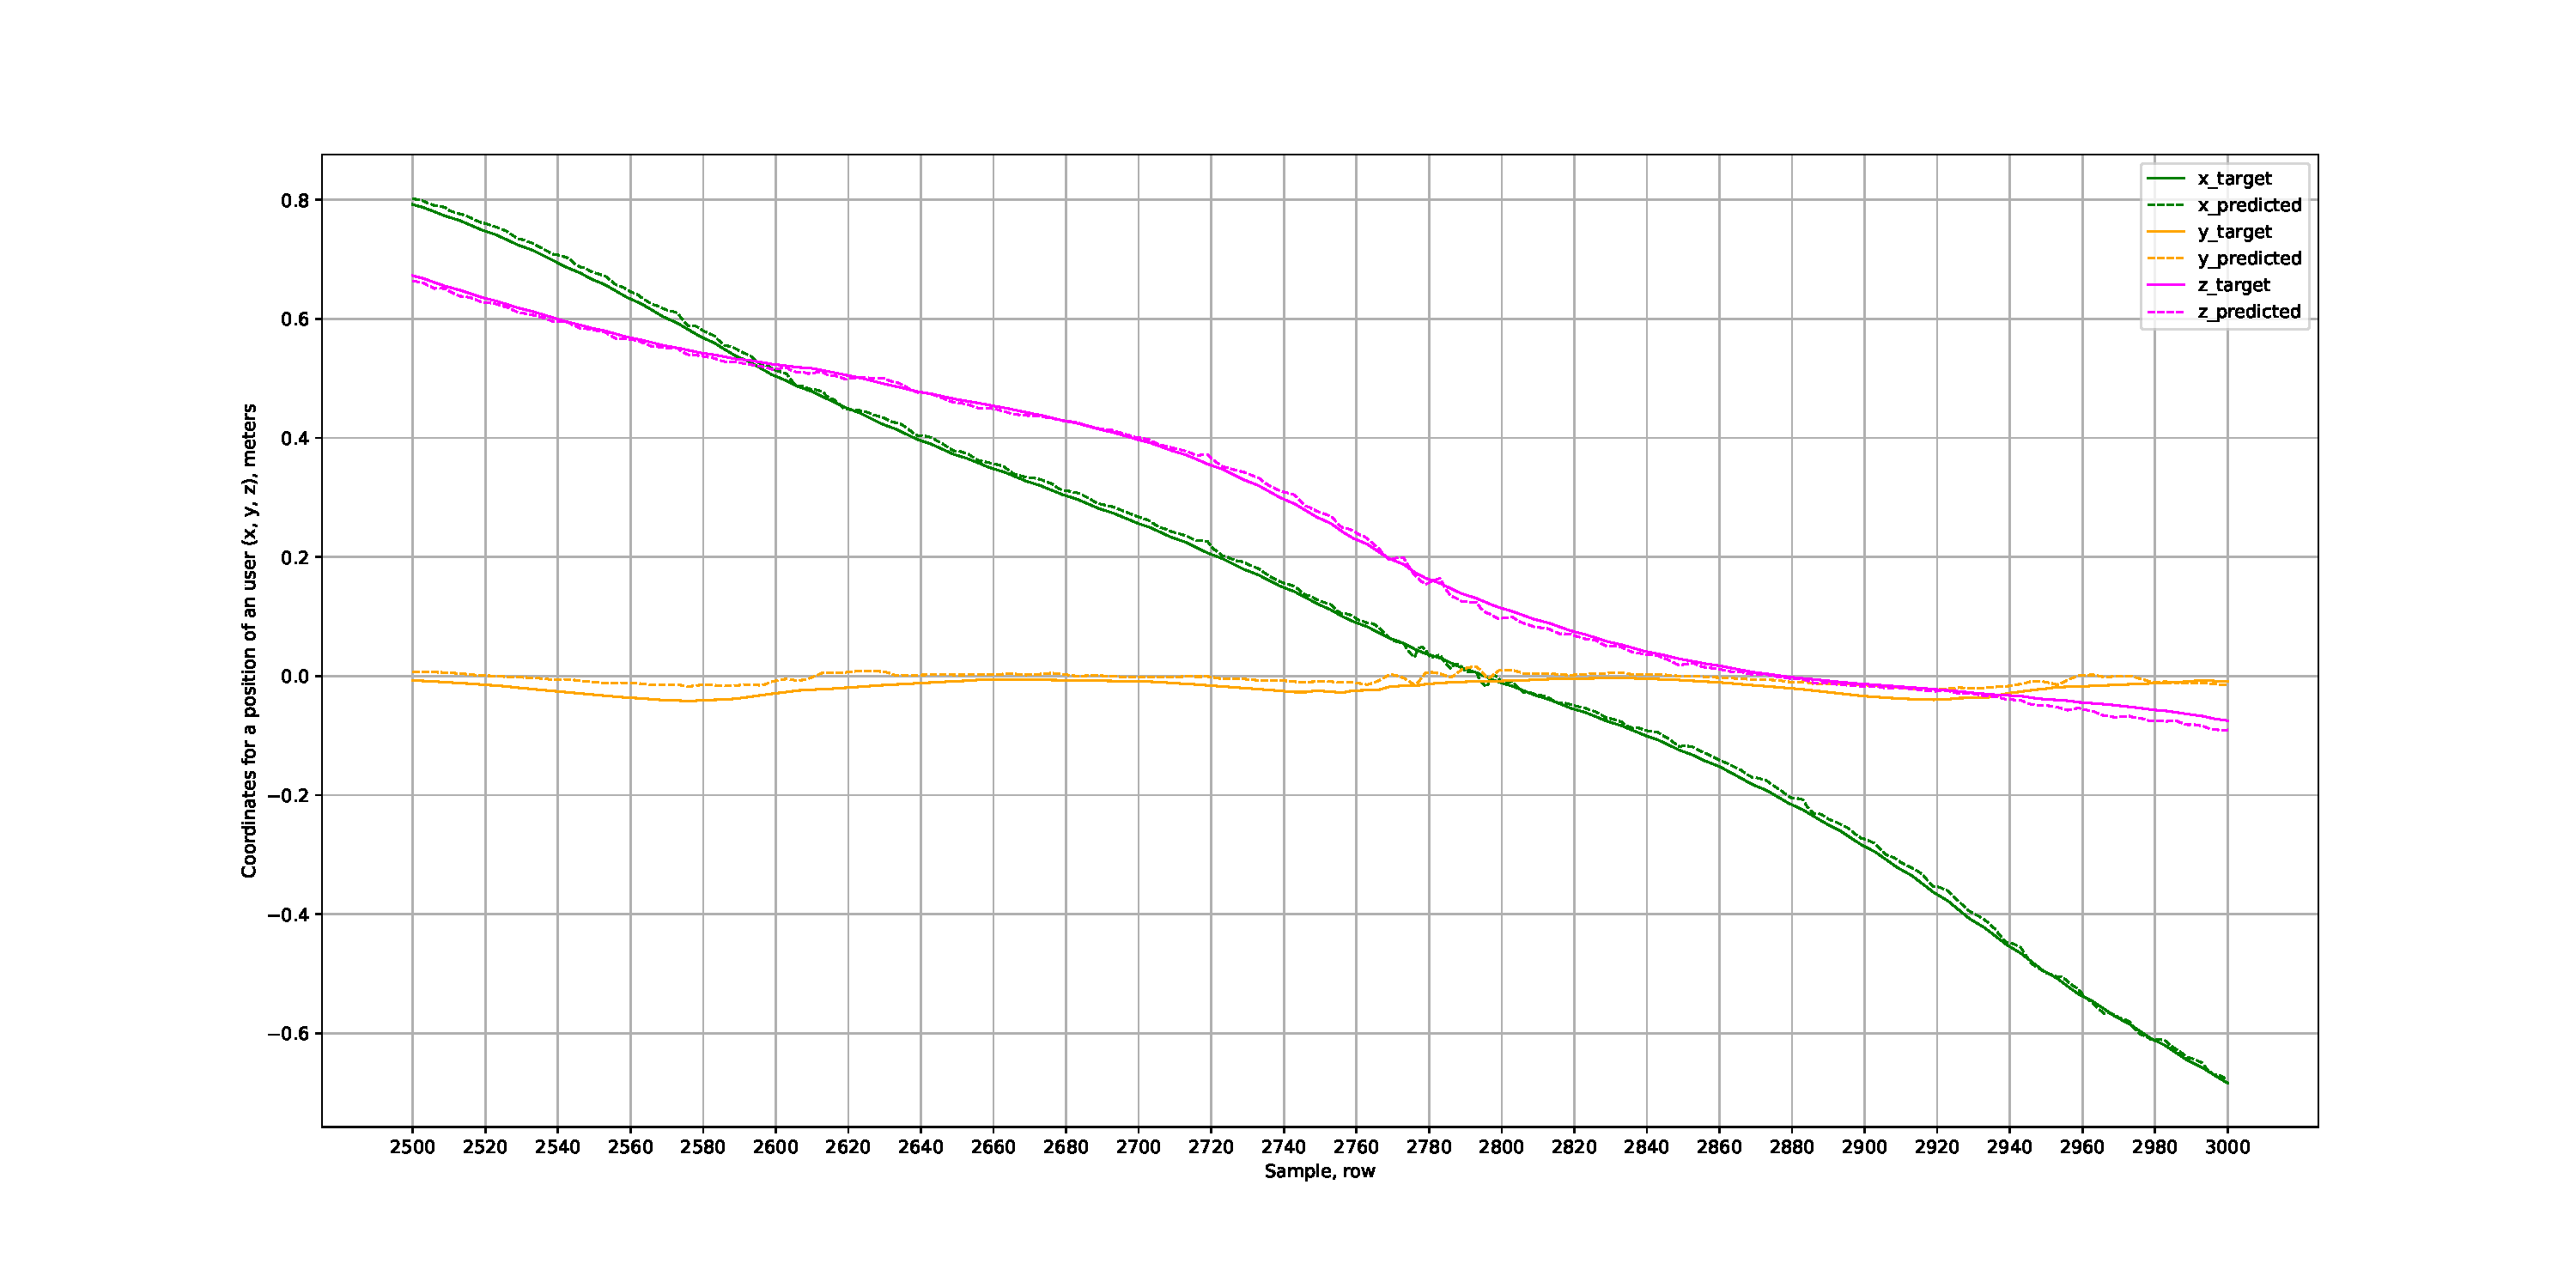
\includegraphics[width=0.9\textwidth, keepaspectratio]{gfx/lstm1_interpolated-xyz_position.pdf}
		\caption{\label{fig:interp1} Outputs of LSTM1 model on interpolated dataset for x, y and z axes.}
	\end{center}
\end{figure}

\begin{figure}
	\begin{center}
		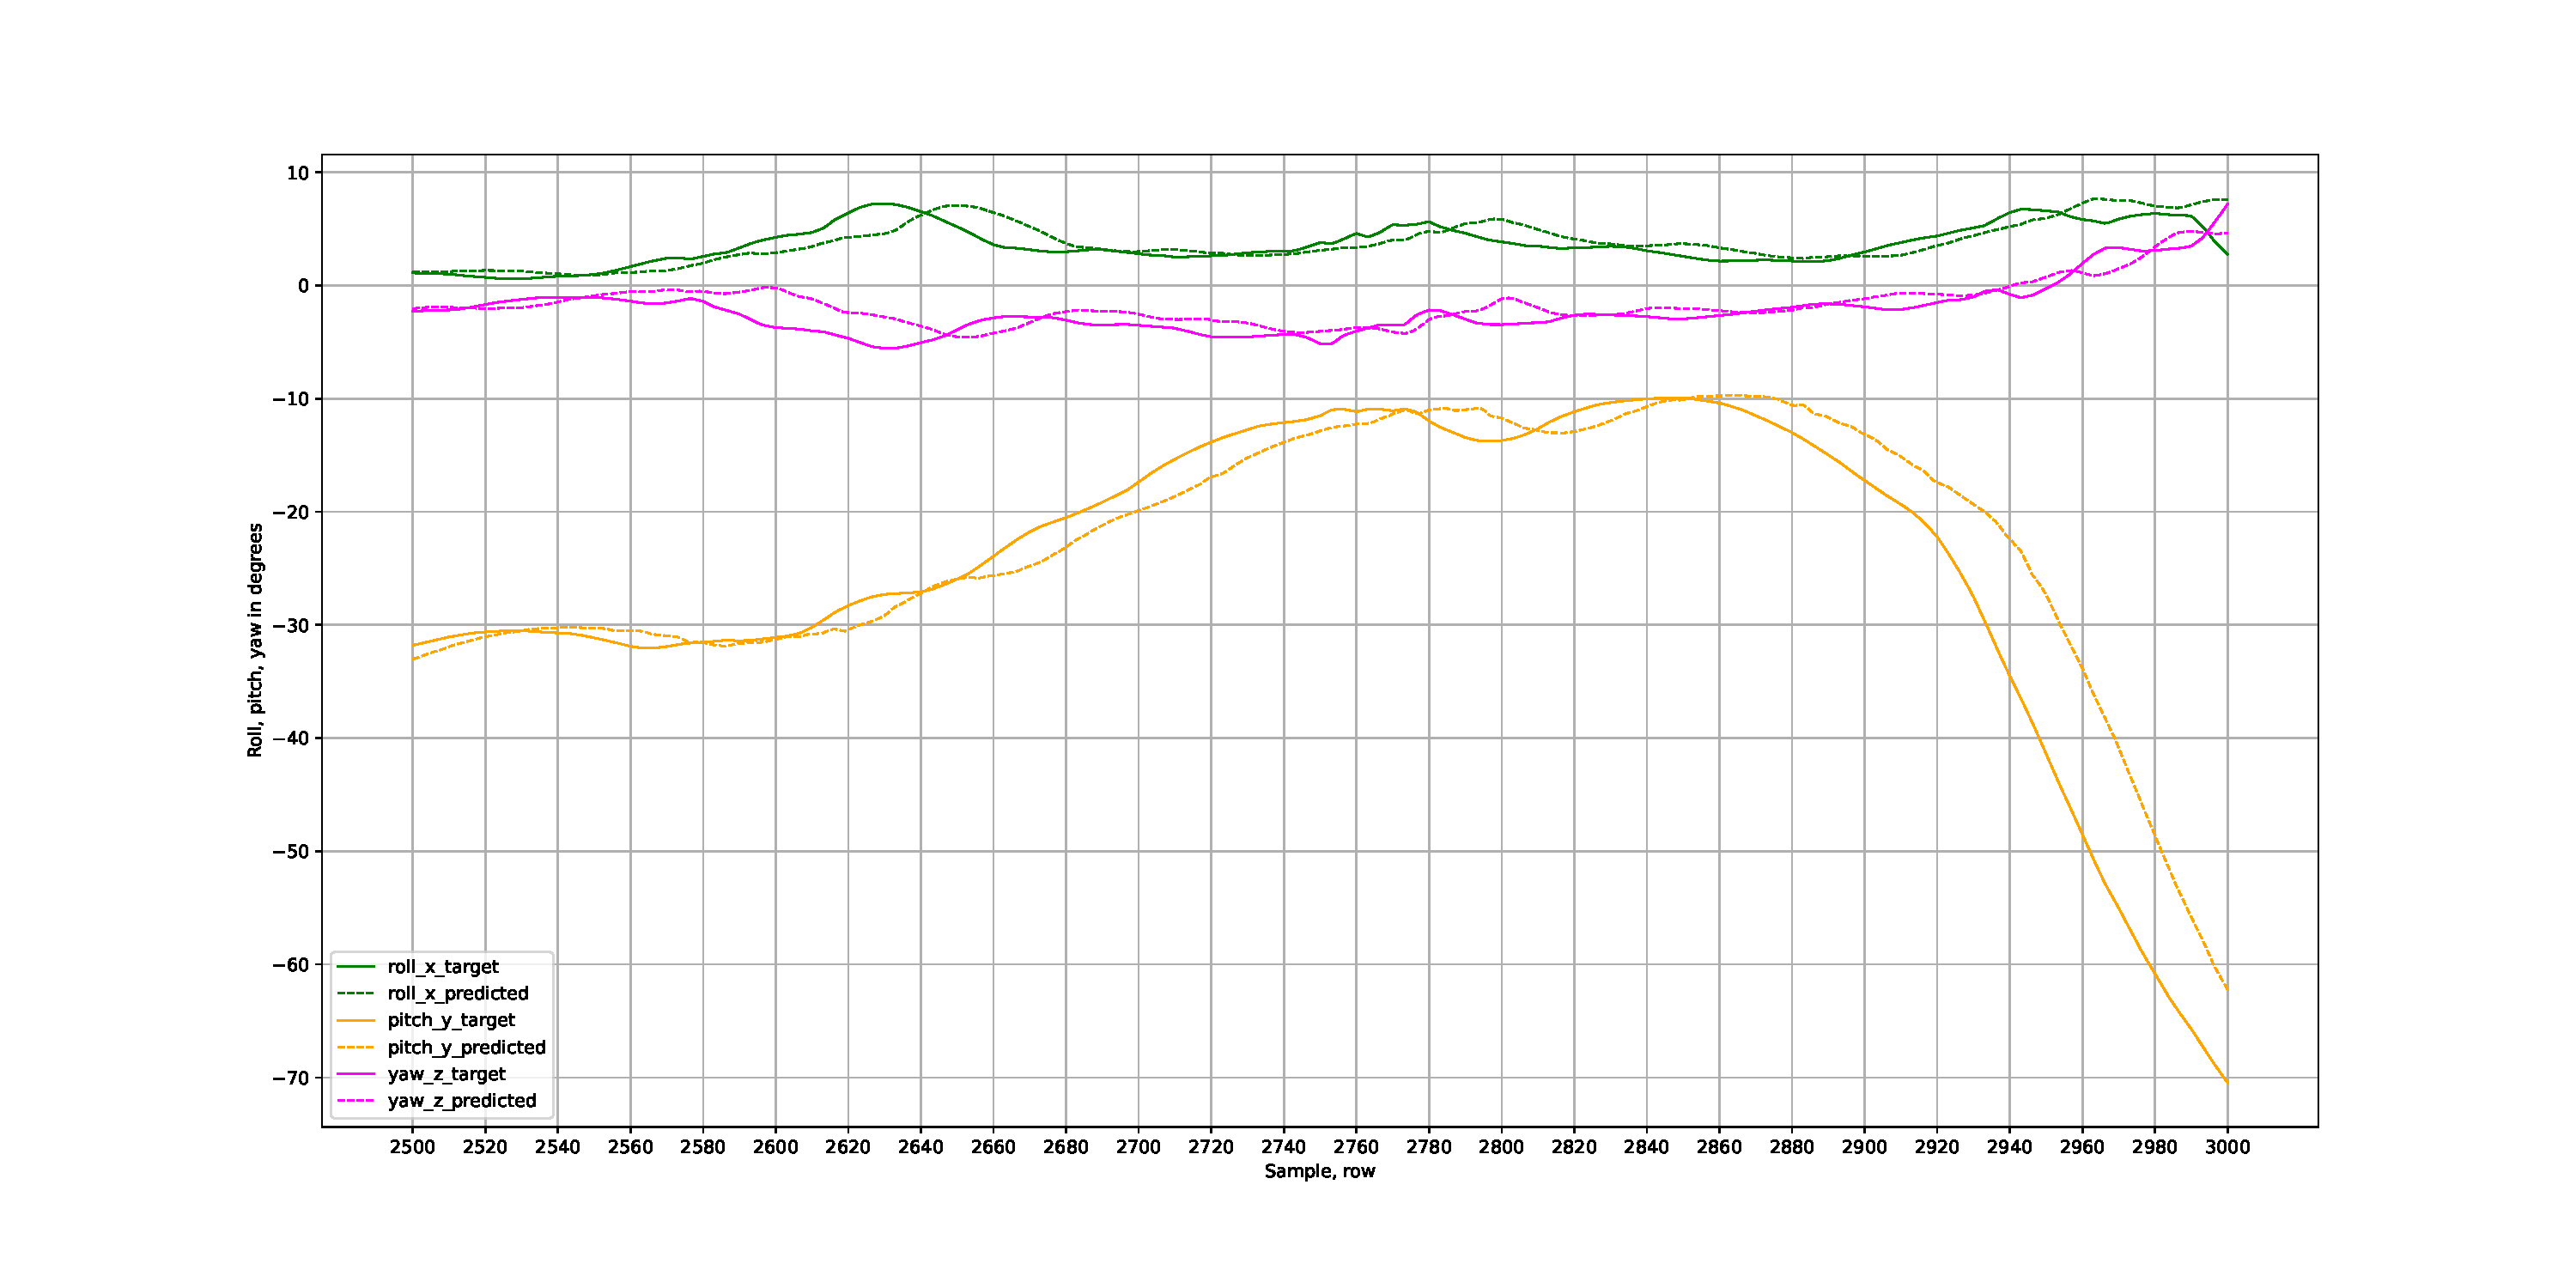
\includegraphics[width=0.9\textwidth, keepaspectratio]{gfx/lstm1_interpolated-roll_pitch_yaw.pdf}
		\caption{\label{fig:interp2} Outputs of LSTM1 model on interpolated dataset for qx, qy, qz and qw axes.}
	\end{center}
\end{figure}

\begin{figure}
	\begin{center}
		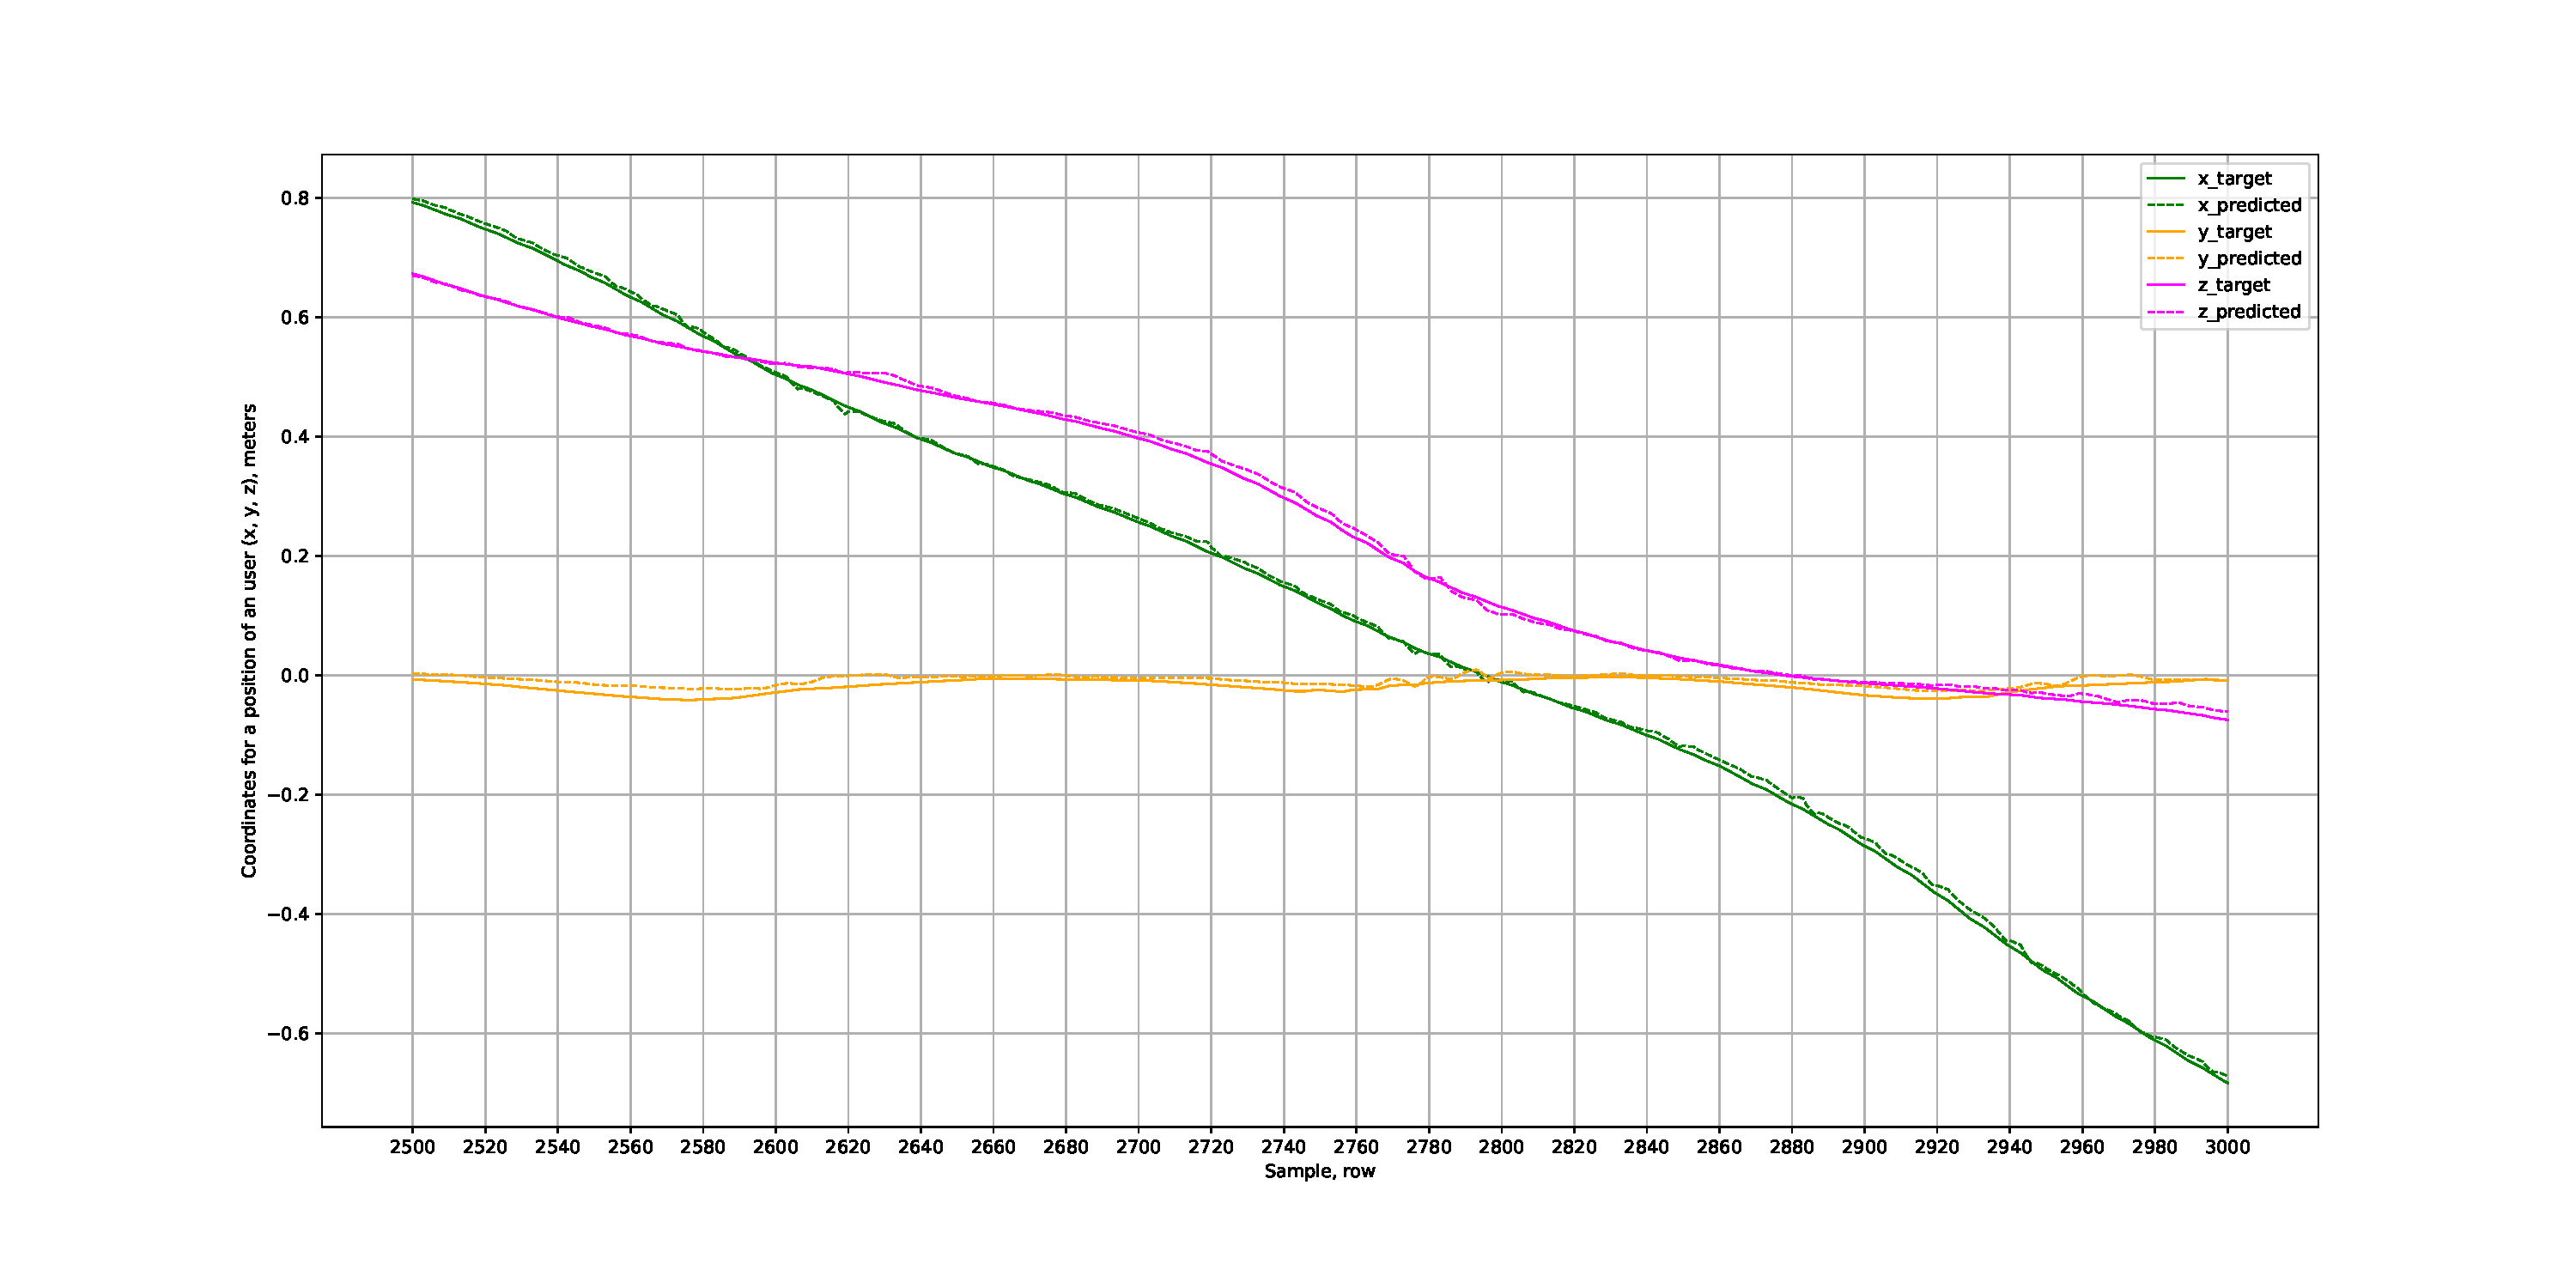
\includegraphics[width=0.9\textwidth, keepaspectratio]{gfx/lstm1_flipped-xyz_position.pdf}
		\caption{\label{fig:flip1} Outputs of LSTM1 model on dataset with flipped negative quaternions for x, y and z axes.}
	\end{center}
\end{figure}

\begin{figure}
	\begin{center}
		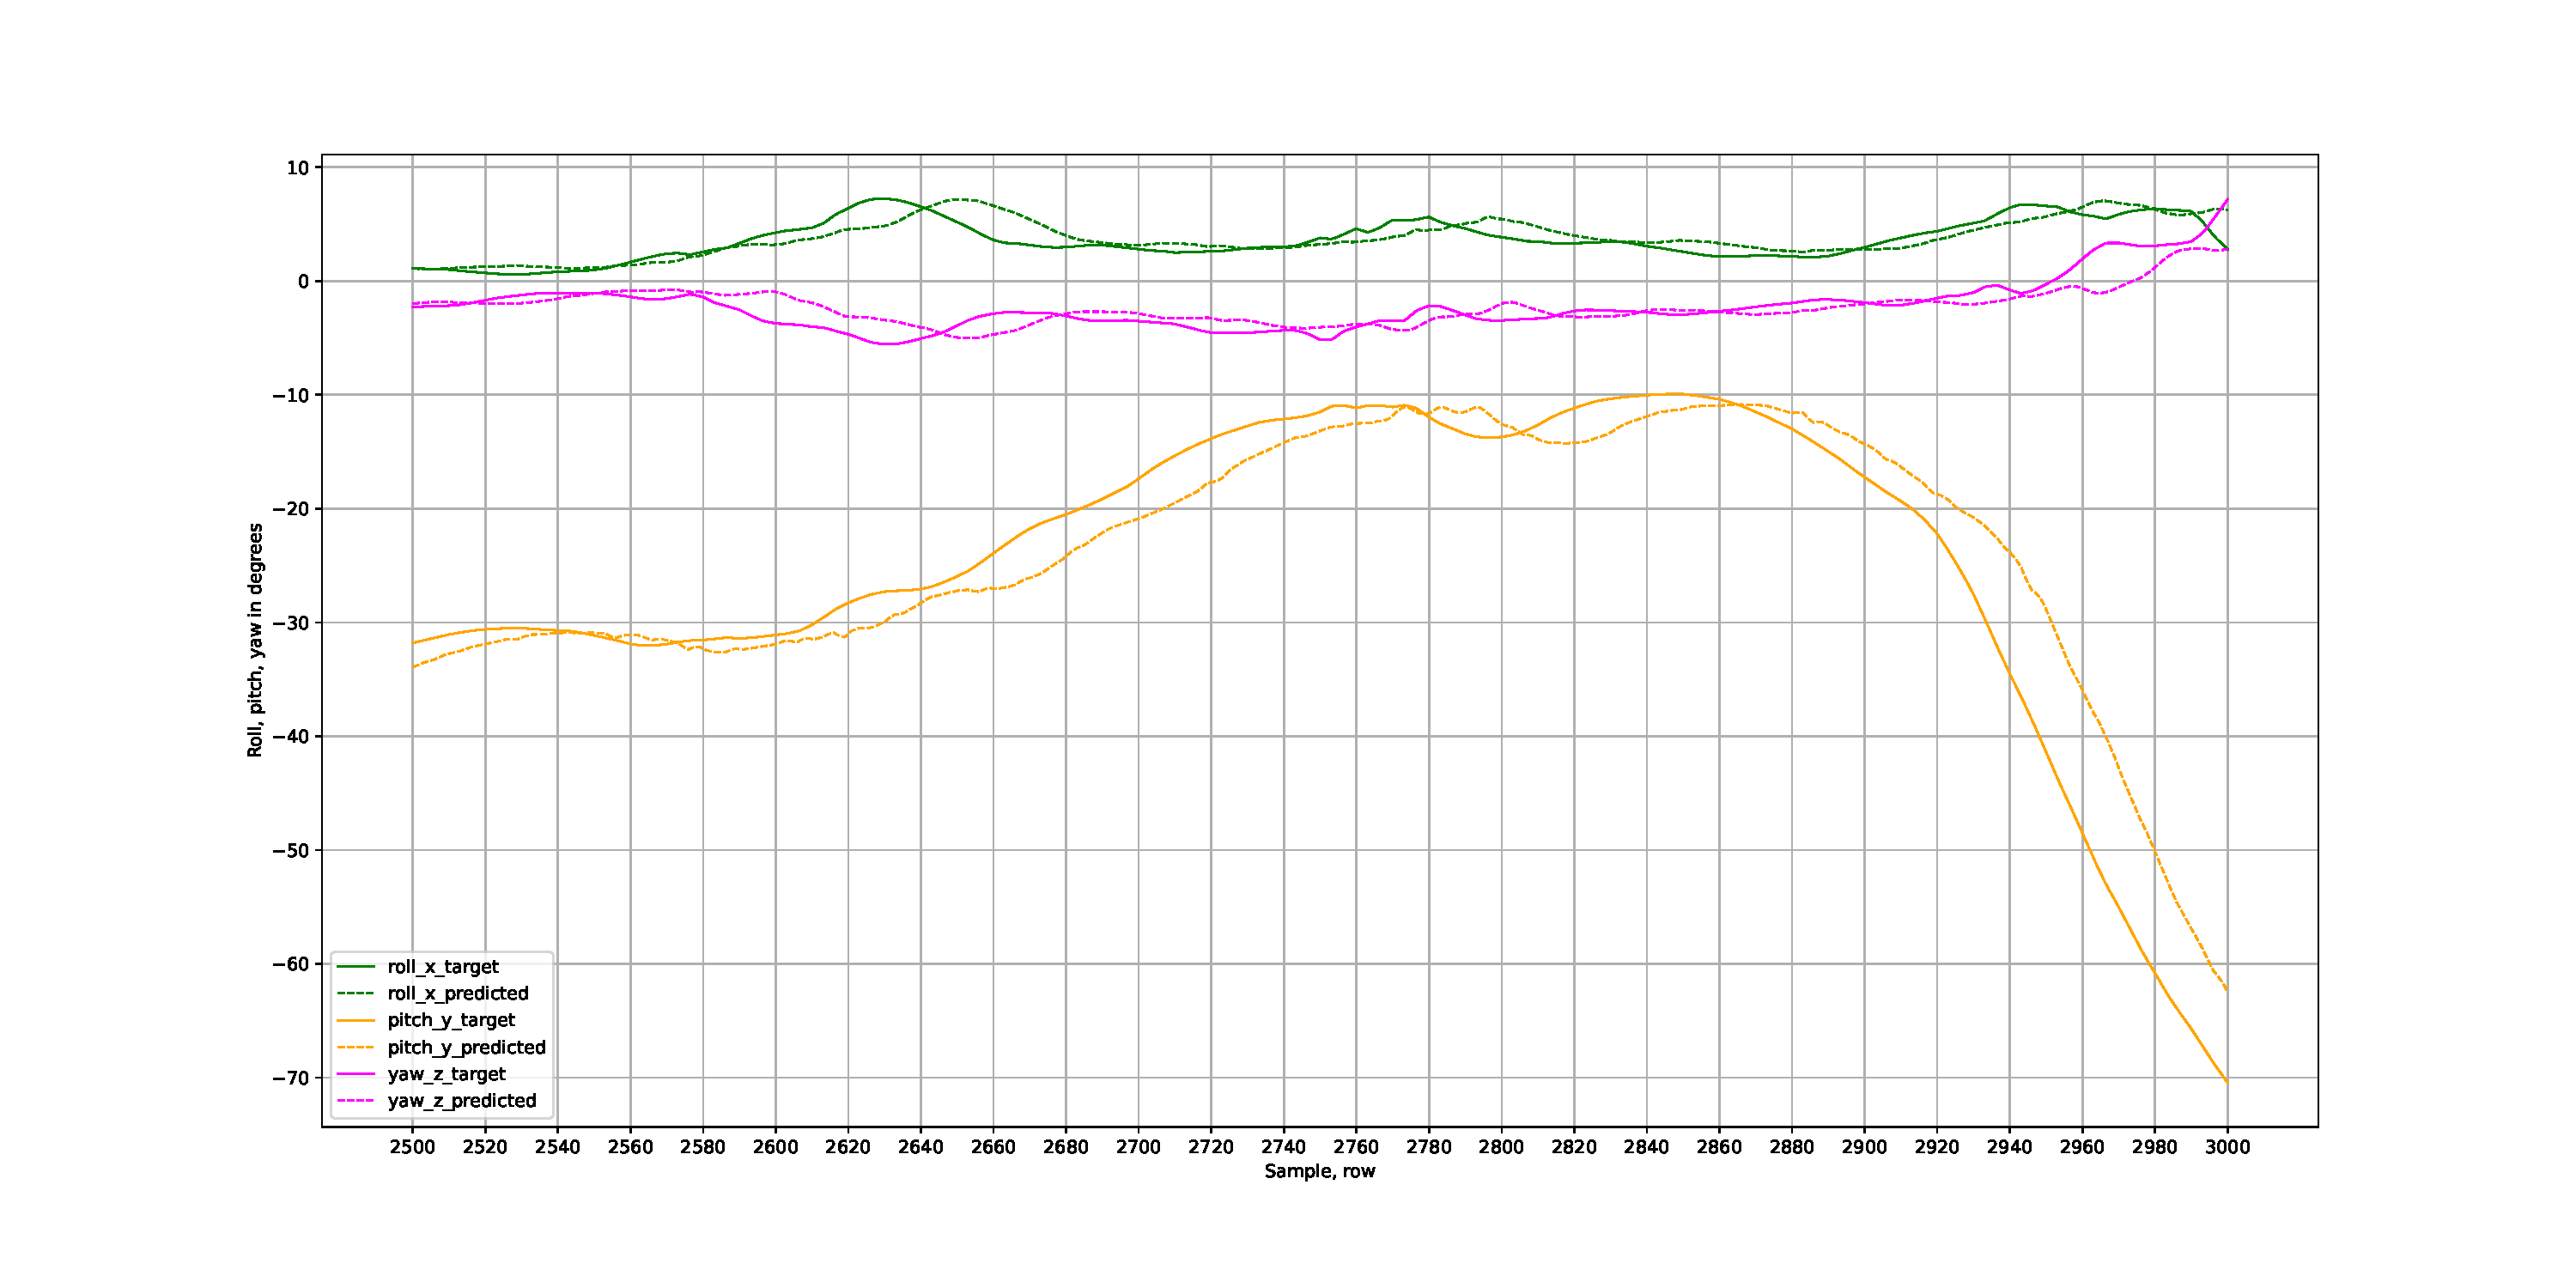
\includegraphics[width=0.9\textwidth, keepaspectratio]{gfx/lstm1_flipped-roll_pitch_yaw.pdf}
		\caption{\label{fig:flip2} Outputs of LSTM1 model on dataset with flipped negative quaternions for qx, qy, qz and qw axes.}
	\end{center}
\end{figure}